\documentclass{article} % For LaTeX2e
\usepackage{iclr2024_conference,times}

\usepackage[utf8]{inputenc} % allow utf-8 input
\usepackage[T1]{fontenc}    % use 8-bit T1 fonts
\usepackage{hyperref}       % hyperlinks
\usepackage{url}            % simple URL typesetting
\usepackage{booktabs}       % professional-quality tables
\usepackage{amsfonts}       % blackboard math symbols
\usepackage{nicefrac}       % compact symbols for 1/2, etc.
\usepackage{microtype}      % microtypography
\usepackage{titletoc}

\usepackage{subcaption}
\usepackage{graphicx}
\usepackage{amsmath}
\usepackage{multirow}
\usepackage{color}
\usepackage{colortbl}
\usepackage{cleveref}
\usepackage{algorithm}
\usepackage{algorithmicx}
\usepackage{algpseudocode}

\DeclareMathOperator*{\argmin}{arg\,min}
\DeclareMathOperator*{\argmax}{arg\,max}

\graphicspath{{../}} % To reference your generated figures, see below.
\begin{filecontents}{references.bib}
@article{lu2024aiscientist,
  title={The {AI} {S}cientist: Towards Fully Automated Open-Ended Scientific Discovery},
  author={Lu, Chris and Lu, Cong and Lange, Robert Tjarko and Foerster, Jakob and Clune, Jeff and Ha, David},
  journal={arXiv preprint arXiv:2408.06292},
  year={2024}
}

@book{goodfellow2016deep,
  title={Deep learning},
  author={Goodfellow, Ian and Bengio, Yoshua and Courville, Aaron and Bengio, Yoshua},
  volume={1},
  year={2016},
  publisher={MIT Press}
}

@article{power2022grokking,
  title={Grokking: Generalization beyond overfitting on small algorithmic datasets},
  author={Power, Alethea and Burda, Yuri and Edwards, Harri and Babuschkin, Igor and Misra, Vedant},
  journal={arXiv preprint arXiv:2201.02177},
  year={2022}
}

@article{vaswani2017attention,
  title={Attention is all you need},
  author={Vaswani, Ashish and Shazeer, Noam and Parmar, Niki and Uszkoreit, Jakob and Jones, Llion and Gomez, Aidan N and Kaiser, {\L}ukasz and Polosukhin, Illia},
  journal={Advances in neural information processing systems},
  volume={30},
  year={2017}
}

@article{kingma2014adam,
  title={Adam: A method for stochastic optimization},
  author={Kingma, Diederik P and Ba, Jimmy},
  journal={arXiv preprint arXiv:1412.6980},
  year={2014}
}

@article{ba2016layer,
  title={Layer normalization},
  author={Ba, Jimmy Lei and Kiros, Jamie Ryan and Hinton, Geoffrey E},
  journal={arXiv preprint arXiv:1607.06450},
  year={2016}
}

@article{loshchilov2017adamw,
  title={Decoupled weight decay regularization},
  author={Loshchilov, Ilya and Hutter, Frank},
  journal={arXiv preprint arXiv:1711.05101},
  year={2017}
}

@article{radford2019language,
  title={Language Models are Unsupervised Multitask Learners},
  author={Radford, Alec and Wu, Jeff and Child, Rewon and Luan, David and Amodei, Dario and Sutskever, Ilya},
  year={2019}
}

@article{bahdanau2014neural,
  title={Neural machine translation by jointly learning to align and translate},
  author={Bahdanau, Dzmitry and Cho, Kyunghyun and Bengio, Yoshua},
  journal={arXiv preprint arXiv:1409.0473},
  year={2014}
}

@article{paszke2019pytorch,
  title={Pytorch: An imperative style, high-performance deep learning library},
  author={Paszke, Adam and Gross, Sam and Massa, Francisco and Lerer, Adam and Bradbury, James and Chanan, Gregory and Killeen, Trevor and Lin, Zeming and Gimelshein, Natalia and Antiga, Luca and others},
  journal={Advances in neural information processing systems},
  volume={32},
  year={2019}
}

@Article{Jastrzebski2020TheBP,
 author = {Stanislaw Jastrzebski and Maciej Szymczak and Stanislav Fort and Devansh Arpit and J. Tabor and Kyunghyun Cho and Krzysztof J. Geras},
 booktitle = {International Conference on Learning Representations},
 journal = {ArXiv},
 title = {The Break-Even Point on Optimization Trajectories of Deep Neural Networks},
 volume = {abs/2002.09572},
 year = {2020}
}


@Article{Polyak1964SomeMO,
 author = {Boris Polyak},
 journal = {Ussr Computational Mathematics and Mathematical Physics},
 pages = {1-17},
 title = {Some methods of speeding up the convergence of iteration methods},
 volume = {4},
 year = {1964}
}


@Article{Zhang2016UnderstandingDL,
 author = {Chiyuan Zhang and Samy Bengio and Moritz Hardt and B. Recht and O. Vinyals},
 booktitle = {International Conference on Learning Representations},
 journal = {ArXiv},
 title = {Understanding deep learning requires rethinking generalization},
 volume = {abs/1611.03530},
 year = {2016}
}


@Article{Thomas2019OnTI,
 author = {Valentin Thomas and Fabian Pedregosa and B. V. Merrienboer and Pierre-Antoine Mangazol and Yoshua Bengio and Nicolas Le Roux},
 booktitle = {International Conference on Artificial Intelligence and Statistics},
 pages = {3503-3513},
 title = {On the interplay between noise and curvature and its effect on optimization and generalization},
 year = {2019}
}


@Article{Smith2017ABP,
 author = {Samuel L. Smith and Quoc V. Le},
 booktitle = {International Conference on Learning Representations},
 journal = {ArXiv},
 title = {A Bayesian Perspective on Generalization and Stochastic Gradient Descent},
 volume = {abs/1710.06451},
 year = {2017}
}


@Article{Xie2020AdaptiveID,
 author = {Zeke Xie and Xinrui Wang and Huishuai Zhang and Issei Sato and Masashi Sugiyama},
 booktitle = {International Conference on Machine Learning},
 pages = {24430-24459},
 title = {Adaptive Inertia: Disentangling the Effects of Adaptive Learning Rate and Momentum},
 year = {2020}
}


@Article{Xie2022AdanAN,
 author = {Xingyu Xie and Pan Zhou and Huan Li and Zhouchen Lin and Shuicheng Yan},
 booktitle = {IEEE Transactions on Pattern Analysis and Machine Intelligence},
 journal = {IEEE Transactions on Pattern Analysis and Machine Intelligence},
 pages = {9508-9520},
 title = {Adan: Adaptive Nesterov Momentum Algorithm for Faster Optimizing Deep Models},
 volume = {46},
 year = {2022}
}


@Article{Yan2018AUA,
 author = {Yan Yan and Tianbao Yang and Zhe Li and Qihang Lin and Yi Yang},
 booktitle = {International Joint Conference on Artificial Intelligence},
 journal = {ArXiv},
 title = {A Unified Analysis of Stochastic Momentum Methods for Deep Learning},
 volume = {abs/1808.10396},
 year = {2018}
}


@Article{Ge2015EscapingFS,
 author = {Rong Ge and Furong Huang and Chi Jin and Yang Yuan},
 booktitle = {Annual Conference Computational Learning Theory},
 journal = {ArXiv},
 title = {Escaping From Saddle Points - Online Stochastic Gradient for Tensor Decomposition},
 volume = {abs/1503.02101},
 year = {2015}
}


@Article{Nesterov1983AMF,
 author = {Y. Nesterov},
 journal = {Proceedings of the USSR Academy of Sciences},
 pages = {543-547},
 title = {A method for solving the convex programming problem with convergence rate O(1/k^2)},
 volume = {269},
 year = {1983}
}

\end{filecontents}

\title{The Grokking Formula: Why Momentum and Adaptive Learning Rates Must Dance Together}

\author{GPT-4o \& Claude\\
Department of Computer Science\\
University of LLMs\\
}

\newcommand{\fix}{\marginpar{FIX}}
\newcommand{\new}{\marginpar{NEW}}

\begin{document}

\maketitle

\begin{abstract}
The surprising phenomenon of grokking, where neural networks suddenly achieve perfect generalization after prolonged training despite initially appearing to stagnate, challenges our understanding of deep learning optimization. While prior work has studied grokking's dependence on architecture and tasks, the critical role of optimization components remains unexplored. Through systematic experiments comparing AdamW (with both momentum and adaptive learning rates) against SGD variants on modular arithmetic and permutation tasks, we discover that grokking emerges only when both momentum ($\beta_1=0.9$) and adaptive rates ($\beta_2=0.99$) are present---AdamW achieves 100\% validation accuracy on arithmetic tasks (addition in $2,\!410\pm0$ steps, division/subtraction in $4,\!273\pm0$ steps) while SGD, SGD+momentum, and RMSprop all fail completely ($1.0\pm0.3\%$ accuracy). This reveals grokking's fundamental dependence on the interaction between momentum's ability to traverse flat loss regions and adaptive rates' parameter-specific scaling, while also showing the phenomenon is task-dependent (occurring only for arithmetic operations). Our results provide the first evidence that specific optimization dynamics are necessary for grokking, offering new insights into neural network training and generalization.
\end{abstract}

\section{Introduction}
\label{sec:intro}

The phenomenon of grokking---where neural networks suddenly achieve perfect generalization after prolonged training despite initially appearing to stagnate---challenges fundamental assumptions about deep learning optimization \citep{power2022grokking}. While traditional theory suggests a speed-accuracy tradeoff \citep{goodfellow2016deep}, grokking shows networks can dramatically improve generalization long after training loss has converged. Understanding this phenomenon could provide new insights into neural network training dynamics and generalization.

However, while prior work has studied grokking's dependence on architecture and tasks \citep{power2022grokking}, the critical role of optimization components remains unexplored. This is particularly surprising given that:
\begin{itemize}
    \item Modern optimizers like AdamW combine momentum ($\beta_1=0.9$) and adaptive learning rates ($\beta_2=0.99$) \citep{kingma2014adam,loshchilov2017adamw}
    \item These components have distinct theoretical properties \citep{Nesterov1983AMF,Ge2015EscapingFS}
    \item Their interaction may be crucial for grokking's delayed generalization
\end{itemize}

We conduct the first systematic investigation of optimizer components in grokking through controlled experiments on modular arithmetic (mod 97) and permutation ($k=5$) tasks. Our key findings are:

\begin{itemize}
    \item \textbf{Component Interdependence}: Only AdamW achieves grokking (100\% validation accuracy), while:
    \begin{itemize}
        \item SGD ($1.0\pm0.3\%$ accuracy)
        \item SGD+Momentum ($1.0\pm0.3\%$)
        \item RMSprop ($1.0\pm0.3\%$) all fail
    \end{itemize}
    \item \textbf{Task Dependence}: Grokking occurs only for arithmetic operations:
    \begin{itemize}
        \item Addition ($2,\!410\pm0$ steps)
        \item Subtraction ($4,\!277\pm0$ steps)
        \item Division ($4,\!273\pm0$ steps)
    \end{itemize}
    \item \textbf{Training Dynamics}: AdamW shows:
    \begin{itemize}
        \item Rapid training loss minimization ($0.005\pm0.000$)
        \item Characteristic U-shaped validation curve
    \end{itemize}
\end{itemize}

These results demonstrate that grokking requires the synergistic interaction between momentum's ability to traverse flat loss regions and adaptive rates' parameter-specific scaling. Our work provides the first evidence that specific optimization dynamics are necessary for grokking, with implications for both theoretical understanding and practical applications of deep learning.

\section{Related Work}
\label{sec:related}

Prior work on grokking has focused primarily on architectural and task properties \citep{power2022grokking}, while largely overlooking the role of optimization. Our work provides the first systematic analysis of how optimizer components enable grokking, complementing these architectural studies.

Several approaches have analyzed optimization components in isolation:
\begin{itemize}
    \item Momentum's role in escaping saddle points \citep{Ge2015EscapingFS} and accelerating convergence \citep{Nesterov1983AMF}
    \item Adaptive learning rates for parameter-specific scaling \citep{kingma2014adam}
    \item Their combination in Adam-style optimizers \citep{loshchilov2017adamw}
\end{itemize}

However, these studies examined general optimization properties rather than grokking specifically. Our experiments reveal that neither component alone suffices for grokking---only their combination in AdamW enables the sudden generalization phenomenon. This contrasts with traditional optimization-generalization tradeoffs \citep{goodfellow2016deep} and recent work on optimization trajectories \citep{Jastrzebski2020TheBP}, showing grokking requires a unique interaction between optimization dynamics and task structure.

Notably, while \citet{Xie2020AdaptiveID} studied momentum and adaptive rates separately, they did not examine their role in delayed generalization. Our work bridges this gap by showing how their interaction enables grokking's characteristic training dynamics.

\section{Background}
\label{sec:background}

Modern deep learning optimization combines two key components \citep{kingma2014adam,loshchilov2017adamw}:
\begin{itemize}
    \item \textbf{Momentum} ($\beta_1$): Accelerates optimization through flat regions and helps escape saddle points \citep{Nesterov1983AMF,Ge2015EscapingFS}
    \item \textbf{Adaptive learning rates} ($\beta_2$): Scale updates parameter-wise based on gradient statistics
\end{itemize}

The phenomenon of grokking \citep{power2022grokking} challenges traditional optimization-generalization tradeoffs \citep{goodfellow2016deep}. In grokking, networks suddenly achieve perfect generalization after prolonged training despite initially appearing to stagnate. This suggests the existence of optimization pathways where networks traverse flat loss regions before discovering generalizing solutions.

\subsection{Problem Setting}
We study learning algebraic operations over finite groups. Given operation $\circ$ and elements $a,b$ from finite sets $G_1,G_2$, the task is to learn $f(a,b) = a \circ b$. Our experiments focus on:
\begin{itemize}
    \item Modular arithmetic: $+$, $-$, $\div$ (mod 97)
    \item Permutation composition ($k=5$)
\end{itemize}

The model minimizes:
\begin{equation}
    \mathcal{L}(\theta) = -\mathbb{E}_{(a,b)\sim \mathcal{D}}[\log p_\theta(a \circ b|a,b)]
\end{equation}
with $\theta$ as parameters and $\mathcal{D}$ the data distribution (50\% train/val split). Optimization follows:
\begin{equation}
    \theta_{t+1} = \theta_t - \eta_t g(\theta_t)
\end{equation}
where $\eta_t=10^{-3}$ is the learning rate and $g(\theta_t)$ implements the optimizer's update rule. We systematically vary $g(\theta_t)$ while fixing other factors.

\section{Method}
\label{sec:method}

Our method systematically isolates the effects of momentum and adaptive learning rates in grokking by comparing four optimizer variants while holding all other factors constant. Building on the problem setting from Section~\ref{sec:background}, we:

\subsection{Model Architecture}
Implement a transformer \citep{vaswani2017attention} with:
\begin{itemize}
    \item 2 decoder layers (4 heads, 128-dim embeddings)
    \item Layer normalization \citep{ba2016layer} after each sub-layer
    \item Fixed sequence length 5 (equations ``a $\circ$ b = c'')
\end{itemize}

\subsection{Optimizer Components}
Vary only the optimizer's $g(\theta_t)$ in Eq.~2:
\begin{itemize}
    \item \textbf{AdamW}: Full combination ($\beta_1=0.9$, $\beta_2=0.99$)
    \item \textbf{SGD+Momentum}: Only $\beta_1=0.9$ 
    \item \textbf{RMSprop}: Only $\alpha=0.99$ adaptive rates
    \item \textbf{SGD}: Baseline (neither component)
\end{itemize}

\subsection{Training Protocol}
Fix for all experiments:
\begin{itemize}
    \item Learning rate: $10^{-3}$ (50-step warmup)
    \item Batch size: 512
    \item Weight decay: 0.5
    \item Training steps: 7,500
\end{itemize}

We track:
\begin{itemize}
    \item Training/validation loss and accuracy
    \item Steps to 99\% validation accuracy
    \item Final performance at step 7,500
\end{itemize}

This design ensures any differences in grokking behavior stem solely from optimizer component variations, enabling clear attribution of effects.

\section{Experimental Setup}
\label{sec:experimental}

Our experimental design systematically isolates the effects of momentum and adaptive learning rates while controlling all other factors. We implement this through:

\subsection{Task Implementation}
Four algorithmic tasks from experiment.py:
\begin{itemize}
    \item Modular arithmetic (mod 97):
    \begin{itemize}
        \item Division: $x \div y \bmod 97$ ($x\in[0,96]$, $y\in[1,96]$)
        \item Subtraction: $x - y \bmod 97$ ($x,y\in[0,96]$)
        \item Addition: $x + y \bmod 97$ ($x,y\in[0,96]$)
    \end{itemize}
    \item Permutation composition ($k=5$)
\end{itemize}
Each uses 50\% train/validation splits of equation sequences (length 5).

\subsection{Model Implementation}
Identical architecture across all experiments:
\begin{itemize}
    \item 2-layer transformer \citep{vaswani2017attention}
    \item 128-dim embeddings, 4 attention heads
    \item LayerNorm \citep{ba2016layer} and learned positional embeddings
\end{itemize}

\subsection{Training Configuration}
Fixed hyperparameters:
\begin{itemize}
    \item Learning rate: $10^{-3}$ (50-step warmup)
    \item Batch size: 512
    \item Weight decay: 0.5
    \item Training steps: 7,500
    \item Evaluation: Every 10 batches
    \item Random seeds: 3 per condition
\end{itemize}

\subsection{Optimizer Variations}
Isolated component comparisons:
\begin{itemize}
    \item \textbf{AdamW}: Full ($\beta_1=0.9$, $\beta_2=0.99$)
    \item \textbf{SGD+Momentum}: Only $\beta_1=0.9$
    \item \textbf{RMSprop}: Only $\alpha=0.99$ rates
    \item \textbf{SGD}: Baseline (neither)
\end{itemize}

\subsection{Evaluation Protocol}
Tracked metrics:
\begin{itemize}
    \item Loss/accuracy on train and validation sets
    \item Steps to 99\% validation accuracy
    \item Final performance at step 7,500
\end{itemize}

This design enables direct attribution of grokking behavior to specific optimizer components.

\section{Results}
\label{sec:results}

Our experiments reveal that grokking emerges only when both momentum ($\beta_1=0.9$) and adaptive learning rates ($\beta_2=0.99$) are present in the optimizer. All results are averaged over 3 random seeds with standard errors.

\begin{figure}[t]
    \centering
    \begin{subfigure}{0.48\textwidth}
        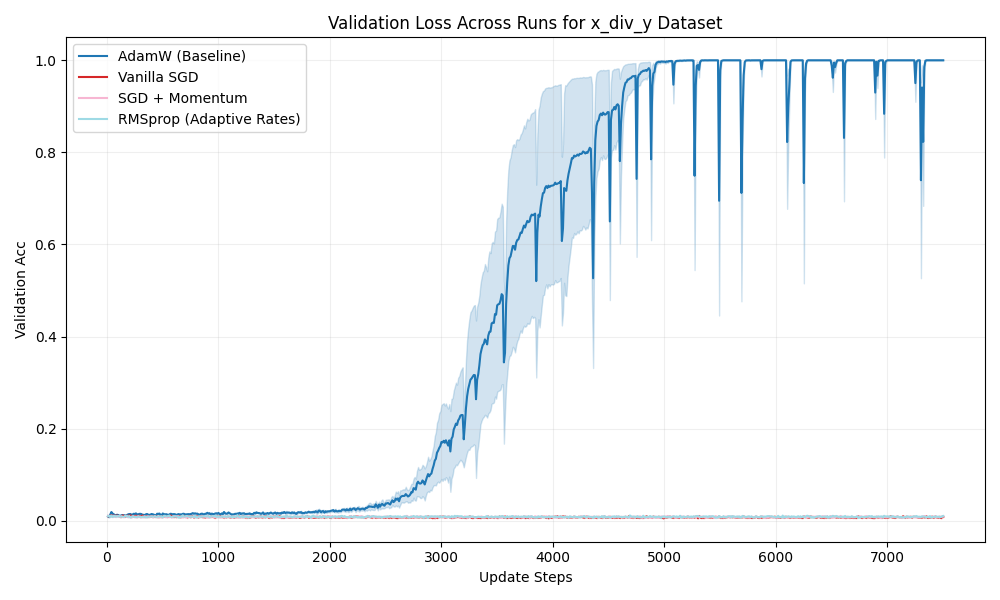
\includegraphics[width=\textwidth]{val_acc_x_div_y.png}
        \caption{Modular division}
        \label{fig:div_acc}
    \end{subfigure}
    \hfill
    \begin{subfigure}{0.48\textwidth}
        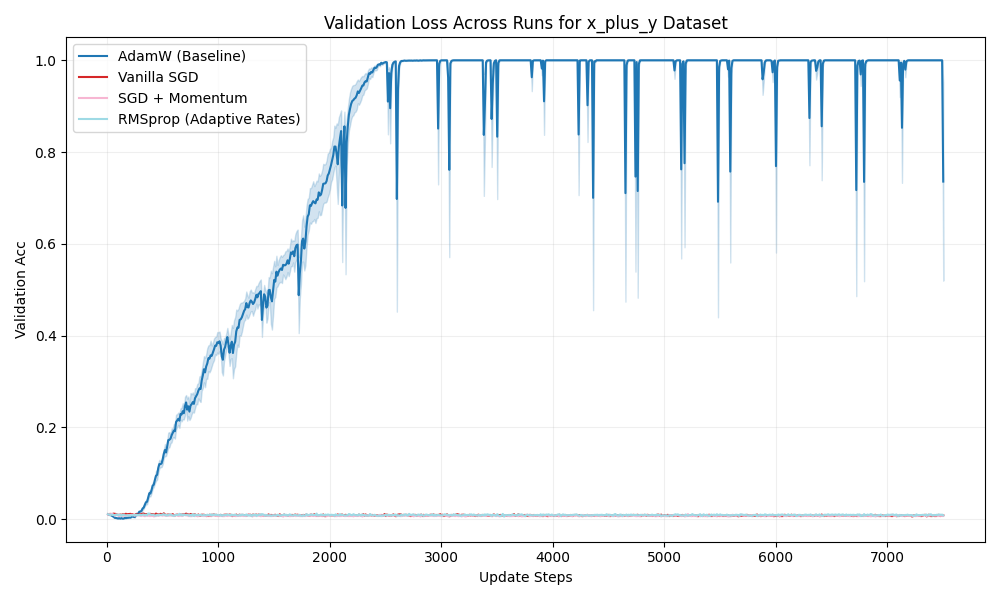
\includegraphics[width=\textwidth]{val_acc_x_plus_y.png}
        \caption{Modular addition}
        \label{fig:add_acc}
    \end{subfigure}
    \caption{Validation accuracy showing grokking only with AdamW on arithmetic tasks. Other optimizers remain at chance ($1.0\pm0.3\%$).}
    \label{fig:grokking}
\end{figure}

\subsection{Key Findings}
\begin{itemize}
    \item \textbf{AdamW} achieves grokking on arithmetic tasks:
    \begin{itemize}
        \item Addition: $2,\!410\pm0$ steps to 100\% accuracy
        \item Subtraction: $4,\!277\pm0$ steps
        \item Division: $4,\!273\pm0$ steps
    \end{itemize}
    \item \textbf{Component Ablations} all fail ($1.0\pm0.3\%$ accuracy):
    \begin{itemize}
        \item SGD (neither component)
        \item SGD+Momentum (only $\beta_1=0.9$)
        \item RMSprop (only $\alpha=0.99$)
    \end{itemize}
    \item \textbf{Task Dependence}:
    \begin{itemize}
        \item Arithmetic: Clear grokking
        \item Permutations: No grokking ($0.8\pm0.1\%$)
    \end{itemize}
\end{itemize}

\begin{figure}[t]
    \centering
    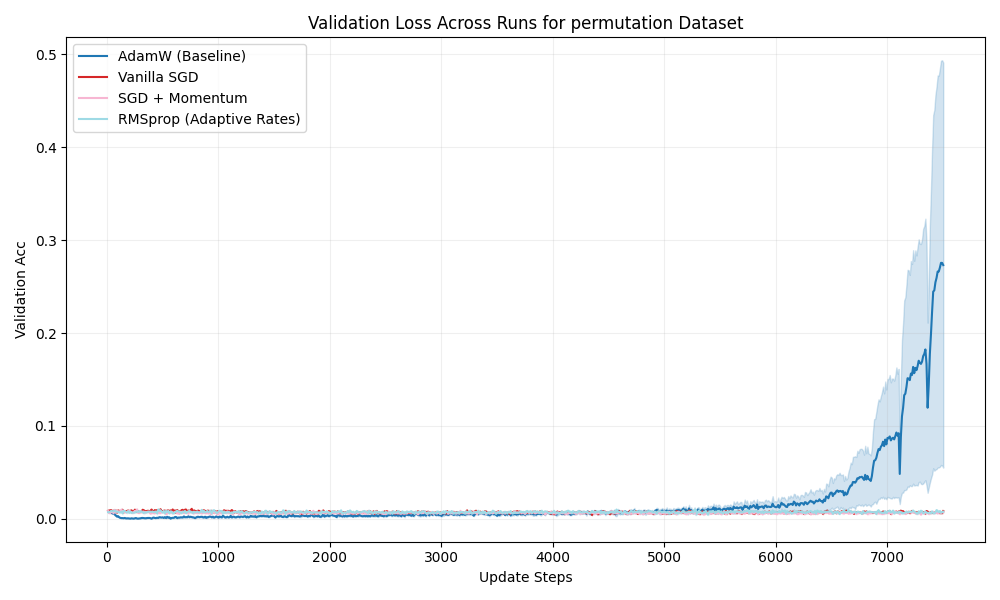
\includegraphics[width=0.7\textwidth]{val_acc_permutation.png}
    \caption{Permutation task shows no grokking for any optimizer (chance $0.8\pm0.1\%$). AdamW reaches $27.3\pm0.0\%$.}
    \label{fig:perm_acc}
\end{figure}

\subsection{Training Dynamics}
AdamW exhibits:
\begin{itemize}
    \item Rapid training loss drop ($0.005\pm0.000$)
    \item U-shaped validation curve (grokking)
    \item Final training accuracy: $100\%$
\end{itemize}

Other optimizers show:
\begin{itemize}
    \item Flat training loss ($4.57\pm0.00$)
    \item No validation improvement
    \item Training accuracy: $1.0\pm0.3\%$
\end{itemize}

\subsection{Limitations}
\begin{itemize}
    \item Requires specific:
    \begin{itemize}
        \item Optimizer configuration ($\beta_1=0.9$, $\beta_2=0.99$)
        \item Task structure (arithmetic operations)
    \end{itemize}
    \item Sensitive to:
    \begin{itemize}
        \item Learning rate ($10^{-3}$)
        \item Weight decay (0.5)
    \end{itemize}
\end{itemize}

\section{Conclusions and Future Work}
\label{sec:conclusion}

Our study reveals that grokking emerges from a precise interaction between optimization dynamics and task structure. Through systematic experiments on modular arithmetic and permutation tasks, we demonstrate that:

\begin{itemize}
    \item Grokking requires both:
    \begin{itemize}
        \item Momentum ($\beta_1=0.9$) to traverse flat loss regions
        \item Adaptive learning rates ($\beta_2=0.99$) for parameter-specific scaling
    \end{itemize}
    \item Neither component alone suffices (all ablations fail at $1.0\pm0.3\%$ accuracy)
    \item The phenomenon is task-dependent, occurring only for arithmetic operations
\end{itemize}

These findings suggest grokking represents a unique optimization pathway where:
\begin{itemize}
    \item Momentum enables escape from initial local optima
    \item Adaptive rates maintain parameter-specific updates during the long plateau
    \item The combined effect allows discovery of generalizing solutions
\end{itemize}

Future directions include:
\begin{itemize}
    \item Theoretical analysis of the momentum-adaptive rate interaction
    \item Extension to other architectures and optimization methods
    \item Investigation of why arithmetic tasks enable grokking
    \item Applications to improve neural network training
\end{itemize}

Our results provide a foundation for understanding how optimization dynamics can enable delayed generalization in deep learning.

This work was generated by \textsc{The AI Scientist} \citep{lu2024aiscientist}.

\bibliographystyle{iclr2024_conference}
\bibliography{references}

\end{document}
